\documentclass[14pt,a4paper]{article}
\usepackage{geometry}
 \geometry{
 a4paper,
 total={170mm,257mm},
 left=30mm,
 right = 30mm,
 top=30mm,
 bottom = 30mm
 }
\usepackage{graphicx}
\usepackage[utf8]{inputenc}
\usepackage[T2A]{fontenc}
\usepackage{minted}
\usepackage{graphicx}
%\DeclareGraphicsExtensions{.pdf,.png,.jpg}
\usepackage{tikz}

\usepackage[backend = biber,language = auto,style = gost-numeric,sorting = none,maxbibnames = 8,maxcitenames = 8]{biblatex}
\usepackage[style=nature,sorting=none,backend=biber,isbn=false,date=year,doi=false,url=true]{biblatex}
\usepackage[russian]{babel}
\graphicspath{ {/home/sahar/Рабочий стол/Tex/новая папка} }
\usepackage{soul}
\usepackage{graphicx}
\usepackage{framed}
\usepackage[normalem]{ulem}\textbf{}
\usepackage{amsmath}
\usepackage{amsthm}
\usepackage{amssymb}
\usepackage{amsfonts}
\usepackage{mathtools}
\usepackage{caption}
\captionsetup{labelsep=period}
\usepackage{enumerate}
\usepackage[utf8]{inputenc}
\usepackage{grffile}
\documentclass{article}
\usepackage{graphicx}

\newtheorem{theorem}{Theorem}
%TO ADD DOTS TO MANUALLY ADDED LIST OF CONTENTS ITEM...
\makeatletter
\patchcmd{\l@section}{\hfil}{%
  \leaders\hbox{$\m@th
    \mkern \@dotsep mu\hbox{.}\mkern \@dotsep
  mu$}\hfill}{}{}
\makeatother
% \usepackage{wrapfig}
\usepackage[
backend=biber,
style=alphabetic,
citestyle=authoryear
]{biblatex}
\usepackage{float} % useful for specifying image location
 %Imports bibliography file
 \addbibresource{library.bib}
% \usepackage[rightcaption]{sidecap}
\title{Семплирование Гиббса}
%\author{Меркушина Анна}
 \usepackage[T2A]{fontenc}
\usepackage[utf8]{inputenc}
\usepackage[russian,english]{babel}


% \bibliography{biblio}   
\usepackage{wrapfig}
\usepackage{subfig}
 \renewcommand{\contentsname}{ОГЛАВЛЕНИЕ}
 
\usepackage{cite}

\usepackage{hyperref}
\renewcommand*\contentsname{Содержание}

\begin{document}
	\pagenumbering{arabic}
	\thispagestyle{empty}
 
 
	\begin{center}
		{\large МОСКОВСКИЙ ГОСУДАРСТВЕННЫЙ УНИВЕРСИТЕТ\\ имени М. В. Ломоносова\\
			\vspace*{1em plus .6em minus .5em}
			Механико - Математический факультет\\
			Кафедра теории вероятностей}
	\end{center} 
	
	\vspace*{13em plus .6em minus .5em}
	\begin{center}
		{\LARGE \textbf{КУРСОВАЯ РАБОТА}}
		
		\bigskip
		
		{\large \textbf {<<Применение семплирования по Гиббсу к задаче о восстановлении многомерного распределения>>}}
	\end{center}
	
	\vspace*{10em plus .6em minus .5em}
	
	\begin{flushright}
		Выполнила студентка группы 308
		\\кафедры теории вероятностей
		\\ Меркушина А. В.
		\[\]
		Научный руководитель:
		\\доктор физико-математических наук, профессор
		\\Яровая Е. Б.
	\end{flushright}
	
	\vspace*{11em plus .4em minus .5em}
	\begin{center}
		Москва, 2020
	\end{center}

	\newpage
 \renewcommand{\contentsname}{Содержание}
\tableofcontents

\newpage
\addcontentsline{toc}{section}{Введение}
\section*{Введение}
Обработка и анализ данных, имеющих пропущенные значения, являются актуальным вопросом прикладной математической статистики. Например, выборки, собранные в больших эпидемиологических исследованиях, зачастую содержат пропущенные значения \cite{la}. При предварительной обработке данных исследователь вынужден либо восстановить пропуск в наблюдениях, либо удалить участника, имеющего потерянное значение. Замена средним, медианой или константой может оказаться некорректной \cite{b}. Также удаление всех наблюдений, связанных с утерянным, часто недопустимо из-за того, что объём выборки может значительно сократиться. По этим причинам в последнее десятилетие развились подходы, задача которых --- восстановить совместное распределение переменных выборки и подобрать для пропущенного значения наиболее правдоподобное заполнение \cite{b}. %\\Например, при исследовании редкого заболевания все имеющиеся наблюдения имеют большую значимость в работе, поэтому удалять все сведения о пациенте при одном отсутствующем --- весомая потеря для исследования.


Цель работы --- изучить теоретическую основу, необходимую для применения метода восстановления пропущенных данных. Для этого в главе 1 сделан краткий обзор метода Монте-Карло, на основе которого будет построен метод восстановления пропущенных значений. В главе 2 приведены необходимые сведения из теории однородных марковских цепей с дискретным числом состояний и марковских процессов с непрерывным множеством состояний, сформулирована эргодическая теорема. В главе 3 приведен алгоритм гиббсовского семплирования \cite{Murphy} --- один из методов Монте-Карло по схеме марковской цепи. Этот метод является одним из теоретических обоснований алгоритма заполнения пропущенных данных. Кроме того, в главе три нами предложен пример применения Гиббсовского семплирования к задаче моделирования выборки из многомерной случайной величины, которую нельзя решить с помощью функциональных преобразований равномерной случайной величины.
%рассматриваются марковские цепи и марковские процессы, которые в паре с методами Монте-Карло позволяют семплировать из потенциально сложного распределения. %Примером сложного распределения на практике является массив данных с множеством зависимых и независимых показателей здоровья.


%В данной работе применяется Гиббсовское семплирование --- один из методов \\Монте-Карло, идея которого заключается в работе с условными распределениями вместо совместных, что значительно снижает трудозатрадность во многих задачах.
   
	\newpage
%	{\LARGE \textbf{Метод Монте-Карло}}\\
%	\vspace*{1em plus .2em minus .2em}
   \section{Метод Монте-Карло}
 
В этой главе мы рассмотрим метод Монте-Карло, широко используемый в статистике. 
%\subsection{Метод Монте-Карло.}
\begin{wrapfigure}{r}{0.43\textwidth}
		\centering
	%	\vspace{-0.7cm}
	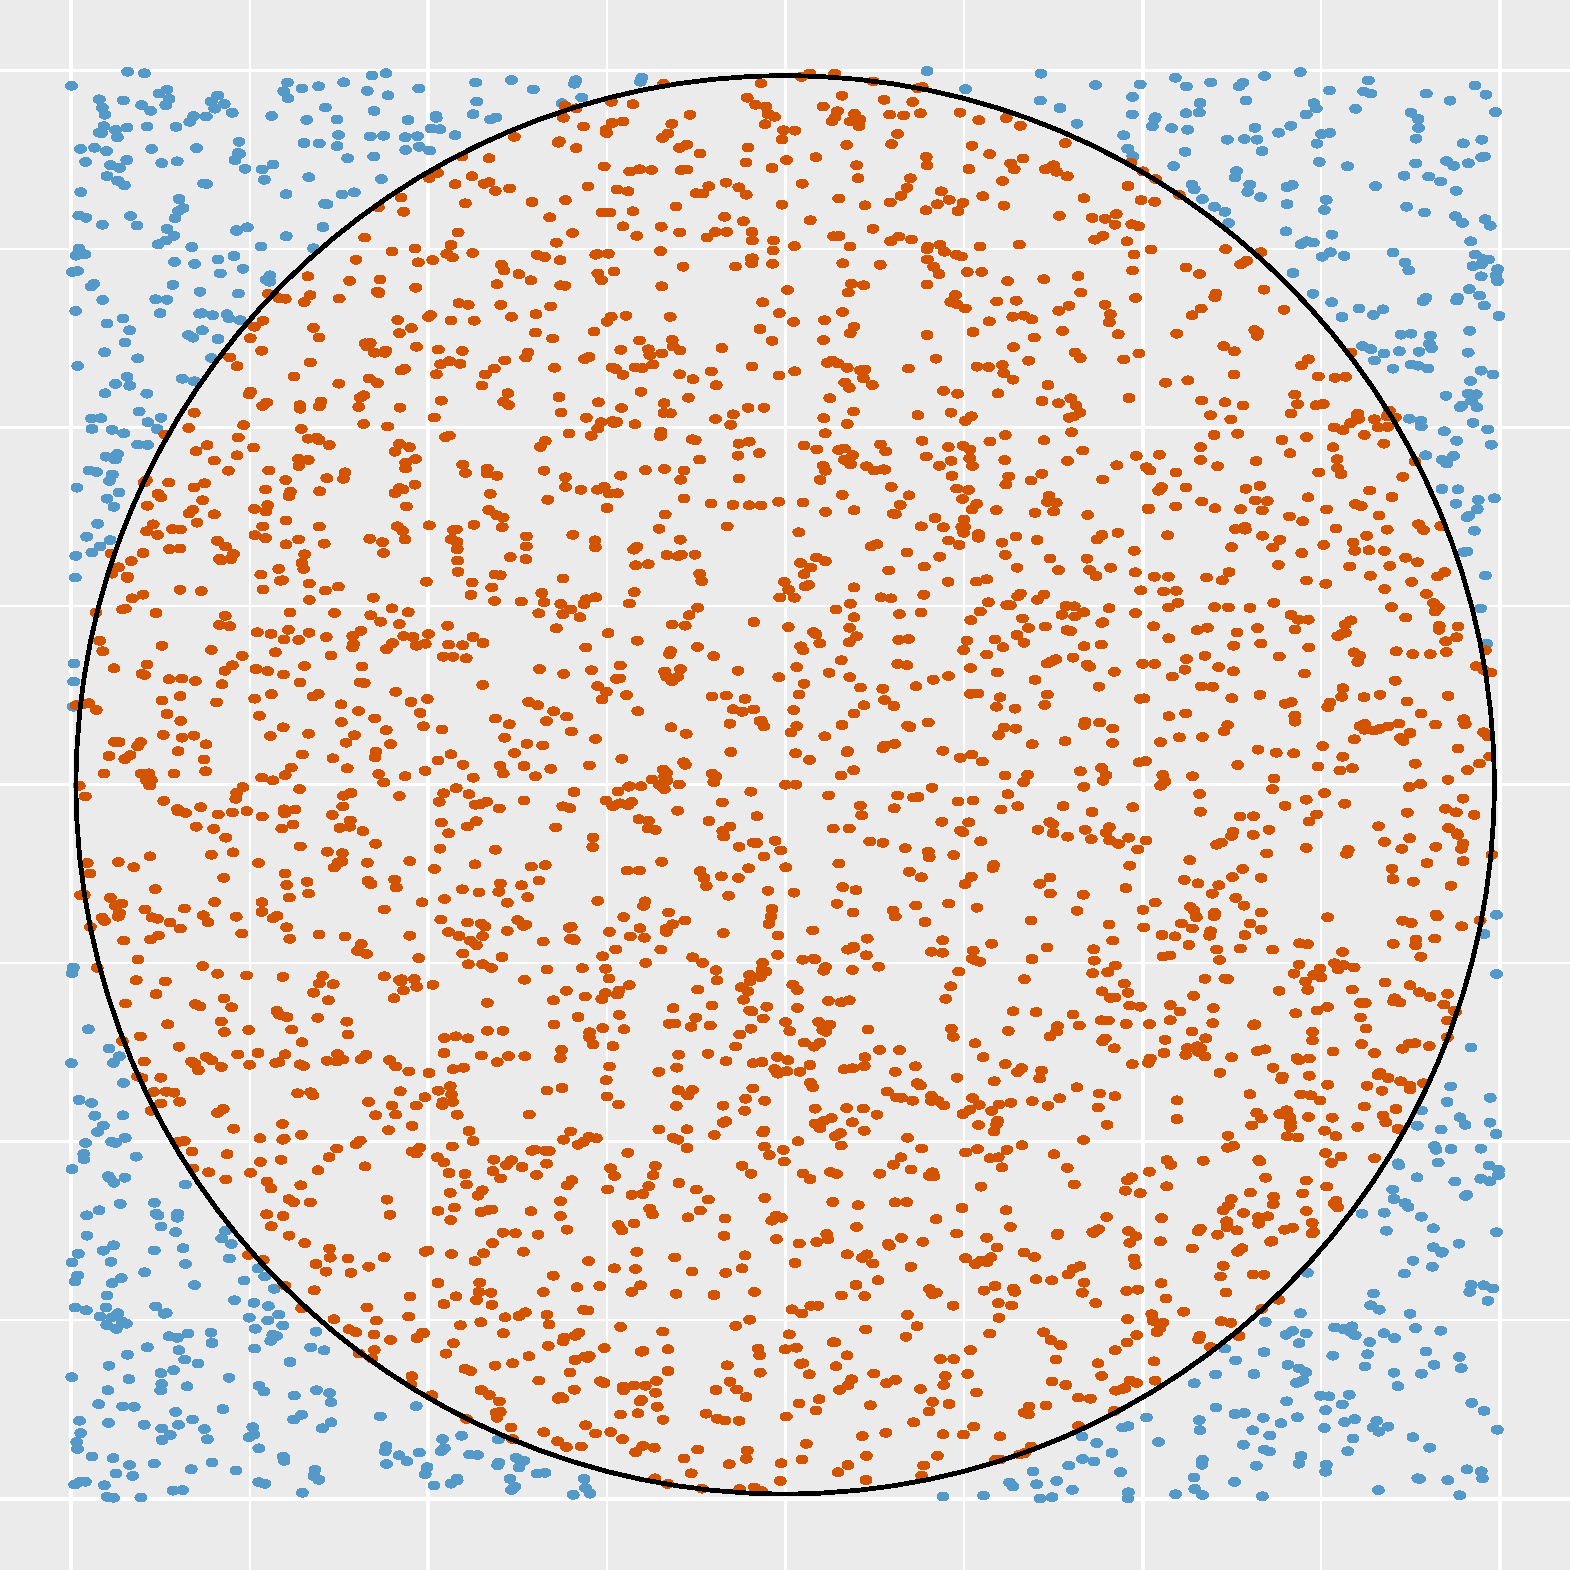
\includegraphics[width=0.43\textwidth]{imgs/Rplot07.pdf}
		\caption{Распределение точек при вычислении числа $\pi$ методом Монте-Карло.}
\end{wrapfigure} 
%\blindtext
\vspace*{3.5em plus .6em minus .5em}

Модельный пример метода --- подсчёт числа $\pi$. Заполним квадрат точками со случайными \\координатами, распределёнными по двумерному равномерному закону. Рассчитаем отношение \\количества точек, попавших в круг, к общему \\количеству точек. 
 Вероятность попадания точки в круг равна отношению площадей круга и квадрата:
\begin{equation}
 \frac{\pi R^2 }{(2R)^2} = \frac{\pi}{4} \simeq \frac{N_0}{N_1}.
\end{equation}
\\Чем больше количество точек, тем ближе полученное значение к значению числа $\pi$ (см. Рис.1). 
%\\Часто бывает удобно получить приближенный ответ с  \\помощью вероятностных методов - методов Монте-Карло.%
	\[\]\[\]	\[\]
%\vspace*{0.5em plus .6em minus .5em}

Метод Монте-Карло был, по-видимому, впервые предложен в работе \cite{phys} для вычисления интегралов посредством генерации случайных величин. Предположим, мы хотим провести вычисление интеграла, аналитическая реализация которого трудоемка. В таком случае часто используются методы численного интегрирования. Для примера рассмотрим метод прямоугольников:
\begin{equation}
I = \int\limits_a^b f(x) dx \cong \frac{(b-a)}{N}  \sum_{k=1}^{N}f(\overset{\wedge}{x}_{k}),    
\end{equation}
где ${x}_{k}$ --- разбиение отрезка $[a,b]$ на равные части, а $\overset{\wedge}{x}_{k} = \frac{(x_{k+1} - x_k)}{2}$ --- произвольно отмеченные точки.

В многомерных задачах численные методы становятся неприемлимыми из-за того, что количество точек разбиений растет как $N^d$, где $d$---размерность пространства. В этом случае можно применить метод Монте-Карло.

В методе Монте-Карло вместо реализации (2) предлагается взять 
\begin{equation}
    \overset{\wedge}I = \frac{(b-a)}{N}  \sum_{k=1}^{N}f({X}_{k}),
\end{equation}
где $X_k$ --- н.о.р. $U[a,b]$ \footnote{независимые одинаково распределенные случайные величины, имеющие равномерное распределение на отрезке $[a,b]$}.

Применяя к $f(X_k)$ ЗБЧ, видим, что $\overset{\wedge}I$ сходится к 
\begin{equation}
    (b-a)\mathbb{E} f({X}_{k}) = (b-a)\int\limits_a^b f(x)\frac{1}{(b-a)} dx = I.
\end{equation}

Таким образом, для пространств больших размерностей количество точек, в которых необходимо посчитать значения функций при использовании метода Монте-Карло значительно меньше, чем при численном интегрировании.
%При рассмотрении многомерной задачи 
%\[
%\int\limits_A f(x_1, \dots, x_k) dx_1 \dots dx_k 
%\]


\newpage
%{\LARGE \textbf{Марковские цепи}}\\
%\vspace*{1em plus .2em minus .2em}
   \section{Необходимые сведения из теории марковских процессов}
 \textit{Случайная последовательность} --- это такое отображение $X: \Omega \rightarrow \mathbb{R}^\infty$, что прообраз $\forall A \in \mathcal{B}(\mathbb{R}^\infty)$ лежит в сигма-алгебре $\mathcal{F}$, то есть $\{\omega: X(\omega) \in A\}$ является элементом $\mathcal{F}$.\\
 
 \textit{Распределение случайной последовательности} --- это набор вероятностей $P\left(X \in B\right)$ для всех $B \in \mathcal{B}(\mathbb{R}^\infty).$
 
 \textit{Конечномерные распределения случайной последовательности} --- это набор вероятностей $p_{t_1, \dots, t_n}\left(B_1, \dots, B_n \right) = P\left(X_{t_1} \in B_1, \dots, X_{t_n} \in B_n\right)$ при $t_i \in \mathbb{N}, B_i \in \mathcal{B}(\mathbb{R}^\infty).$
  %\[\]
  В случае последовательностей целочисленных случайных величин задаём их распределение с помощью набора вероятностей $p_{i_1, \dots, i_n} = P(X_1 = i_1, \dots, X_n = i_n)$. 
  
   \subsection{Сведения из теории марковских цепей}
   
%  \\Кроме того, совместное распределение дискретного вектора $X_1, \dots, X_n$ для $\forall n, i_1, \dots, i_n$ : 
  %\begin{equation*}\label{eq:pareto mle2}
  %\begin{aligned}
 % P(X_1 = i_1, \dots, X_n = i_n) = P(X_n = i_n | X_{n-1} = i_{n-1}\dots, X_1 = i_1)   
 %\end{aligned} \end{equation*}БРЕД ДОВЕСТИ ДО УМА, так как :
 % \begin{equation} 
%\begin{gathered}
 % P(X_1 = i_1, \dots, X_n = i_n) = P(X_n = i_n | X_{n-1} = i_{n-1}\dots, X_1 = i_1) \times  P(X_{n-1} = i_{n-1}\dots, X_1 = i_1) = \\P(X_n = i_n | X_{n-1} = i_{n-1}\dots, X_1 = i_1) \times  P(X_{n-1} = i_{n-1} | X_{n-2} = i_{n-2} \dots, X_1 = i_1) \times P(X_{n-2} = i_{n-2}\dots, X_1 = i_1) = \\
%\end{gathered} \end{equation}
 %\[\]   

  Случайная последовательность $X_n$, принимающая значения из конечного или счётного множества $S$, называется \textit{марковской цепью} \cite{fell}, если выполняется \textit{марковское свойство}:


\begin{equation}
P(X_n = i_n|X_{n-1} = i_{n-1},\dots, X_{0}=i_{0}) = P(X_n = i_n|X_{n-1} = i_{n-1})= p_{i_{n-1} i_n},
\end{equation}	
$\forall \ n = 0, 1,\dots$ и $\forall \ i_0,\dots, i_n \in S$ с $P(X_{n-1} = i_{n-1},\dots, X_{0}=i_{0})>0$,
\\то есть любое испытание зависит от предшествующего и только от него.
%\[\]

%Поясним:
% \begin{equation} 
%\begin{gathered}
%P(X_n = i_n|X_{n-1} = i_{n-1},\dots, X_{0}=i_{0}) = \frac{P(X_0 = i_0, \dots, X_n = %i_n)}{P(X_{0}= i_{0}, \dots, X_{n-1}= i_{n-1})}.
%\end{gathered} 
%\end{equation}
%Заметим, что ввиду зависимости события в МЦ только от предыдущего последнее выражение можно переписать как:
%\begin{equation}
 %   \frac{p_{0}(i_0)\times \dots\times p_{n}(i_{n-1}, i_n)}{p_{0}(i_0)\times \dots\times %p_{n-1}(i_{n-2}, i_{n-1})} = p_{n}(i_{n-1}, i_n).
%\end{equation}
%И аналогично:
 %\begin{equation} 
%\begin{gathered}
%P(X_n = i_n|X_{n-1} = i_{n-1}) = \frac{P(X_{n-1} = i_{n-1} , X_n = i_n)}{P(X_{n-1}= i_{n-1}) },
%\end{gathered} 
%\end{equation}
%где последнее выражение:
%\begin{equation}
 %   \frac{p_{n-1}(i_{n-2}, i_{n-1})\times  p_{n}(i_{n-1}, i_n)}{ p_{n-1}(i_{n-2}, i_{n-1})} = p_{n}(i_{n-1}, i_n).
%\end{equation}
%\[\]

Если вероятность перехода марковской цепи не зависит от $n$, то цепь \textit{однородна по времени}, т.е. все переходные вероятности не меняются со временем.


Говорят,что из состояния $i$ \textit{следует} состояние $j$, если $\exists$ $n :$ \begin{equation}P(X_n = j|X_0 = i)>0,\end{equation}  
т.е. находясь в состоянии $i$ возможно оказаться в $j$.
%\[\]


Матрица $\mathbf{P}$  называется \textit{стохастической}, если $\forall i, j \ 0 \leqslant p_{ij} \leqslant1$ и $\sum_j p_{i j} = 1 \ \forall i.$

%\footnote{Матрица $\mathbf{P}$ стохастическая, если $\forall i, j \ 0 \leqslant p_{i,j} \leqslant1$ и $\sum_j p_{i,j} = 1 \ \forall i.$}(почему тут вылезла 2?)
\textit{Распределение марковской цепи} определяют:
\begin{itemize}
\item переходная стохастическая матрица цепи $\mathbf{P} = \left(P(X_t = i | X_{t-1} = j)\right) =\left(p_{j i}\right)$,
\item первоначальное распределение, т.е. распределение вероятностей в момент времени $t = 0$:  
\end{itemize}	
%{\centering
\begin{equation}
   \mu = (\mu_1, \dots, \mu_n) = (P(X_0 = i_0))= \left(P\left(X_0 = 1\right),\dots,P\left(X_0 = N\right)\right), 
\end{equation}
так что $\forall \ n = 0, 1,\dots$ и $\forall \ i_0, \dots, i_n \in S$:
\begin{equation}
    P(X_0 = i_0, \dots, X_n = i_n) = \mu_{i_0}p_{i_0 i_1},\dots,p_{i_{n-1} i_n}.
\end{equation}
%\[\]


Увидим закономерность в преобразовании распределений.\\Рассмотрим распределение на 1-ом шаге:
\begin{equation}
\begin{gathered}
    p^{(1)} = (p^{(1)}_1,\dots,p^{(1)}_n) = (\mu_1p_{1,1}+\dots+\mu_n p_{n,1}, \mu_1p_{1,2}+\dots) = \\(\mu_1, \dots, \mu_n)
  \begin{pmatrix}
    p_{1,1} & p_{1,2} & \dots \\
    p_{2,1} & \ddots \\
    \vdots &  \\
  \end{pmatrix} = \mu \mathbf{P}.
\end{gathered}
\end{equation}
Таким образом, распределение на t-ом шаге:
\begin{equation}
    p^{(t)} = (p^{(t)}_1,\dots,p^{(t)}_n) = (P(X_t = i_t))  = \mu \mathbf{P}^t.
\end{equation}
%\par} 

\[\]
Цепь называется \textit{неразложимой (неприводимой)}, если $\forall i, j$ из $i$ следует $j$, а из $j$ следует $i$,\\
иначе говоря, любые состояния $i_a, i_b \in S$ сообщаются, т.е. $\exists n:$
\begin{equation}
    P(X_{m+n} = i_a|X_m = i_b) > 0.
\end{equation}


\begin{figure}[H]
    \centering
    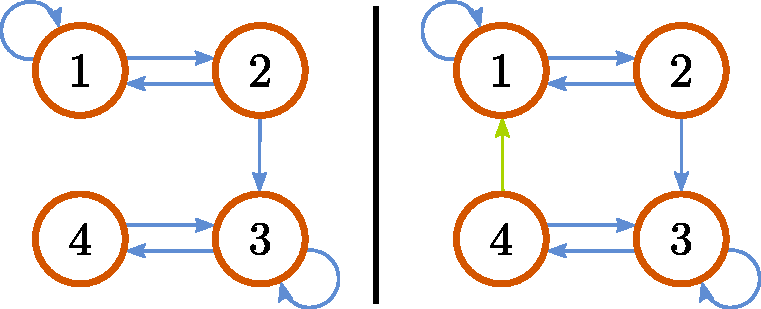
\includegraphics[width=0.56\textwidth]{chain11.pdf}
    \caption{Примеры разложимой (слева) и неразложимой (справа) цепей.}
    \label{fig:my_label}
\end{figure}
% \vspace*{1.5em plus .6em minus .5em}

 Неразложимая цепь называется \textit{непериодической}, если наибольший общий делитель длин замкнутых путей в этой цепи равен 1. Иначе говоря, есть несколько путей из каких-либо состояний в себя, длины которых взаимно просты.

\begin{figure}[H]
    \centering
    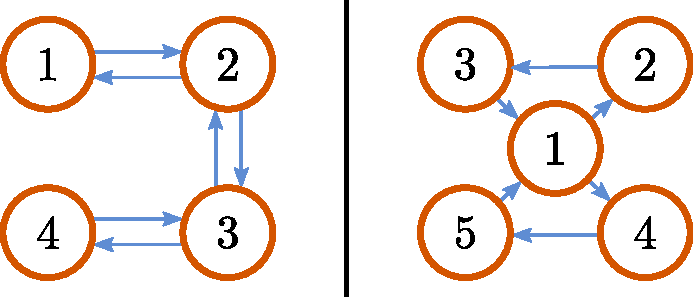
\includegraphics[width=0.50\textwidth]{chain22.pdf}    \caption{Примеры периодичных цепей: слева с периодом k = 2, справа с k = 3.}
    \label{fig:my_label}
\end{figure}
%\end{itemize}
Сведения, изложенные в пункте 2.1 будут использованы в следующем разделе. 



\newpage
\subsection{Эргодическая теорема}
Рассмотрим однородную марковскую цепь с двумя состояниями 0 и 1, которая задается матрицей переходных вероятностей
\begin{equation}
    \mathbf{P} = 
    \begin{pmatrix}
    p_{1 1} & p_{1 2} \\
    p_{2 1} & p_{2 2} \\
  \end{pmatrix}.
\end{equation}
Если в выражении (10) положить $t = n$, то по индукции получаем
\begin{equation}
    \mathbf{P}^n = \frac{1}{2-p_{1 1}-p_{2 2}}
    \begin{pmatrix}
    1 - p_{2 2}& 1 - p_{1 1} \\
        1 - p_{2 2}& 1 - p_{1 1} \\
  \end{pmatrix} + \frac{(p_{1 1}+p_{2 2}-1)^n}{2-p_{1 1}-p_{2 2}}
    \begin{pmatrix}
    1 - p_{1 1}& -(1 - p_{1 1}) \\
        -(1 - p_{2 2})& 1 - p_{1 1} \\
  \end{pmatrix}.
\end{equation}
В выражении (13) устремим $n \to \infty$, тогда
\begin{equation}
    \mathbf{P}^n \to
    \frac{1}{2-p_{1 1}-p_{2 2}}
    \begin{pmatrix}
    1 - p_{2 2}& 1 - p_{1 1} \\
        1 - p_{2 2}& 1 - p_{1 1} \\
  \end{pmatrix}.
\end{equation}
Таким образом, с течением времени $p_{j i}^{(n)}$ сходятся к предельным значениям $\pi_i$, не зависящим от j \cite{shir}.
\[\]
Далее приведем теорему из работы \cite{shir}.
\newtheorem{Th}{Теорема}
\begin{Th}%[koko]
Если конечная цепь Маркова с переходной матрицей $\mathbf{P}$ является неразложимой и апериодичной, то при любом начальном распределении $\lambda$ вероятности $P(X_n = i)$ сходятся к некоторым $\pi_i$, $i = 1,\dots,N$ при $n\rightarrow\infty$:
\begin{equation}
    \mathbf{P}^n \rightarrow\ \mathbf{\Pi}, n\rightarrow\infty.
\end{equation}

При этом вектор $\pi = (\pi_1,\dots,\pi_N)$ является единственным решением системы уравнений 
\begin{equation}
    \pi \mathbf{P} = \pi 
\end{equation}
и называется \textit{эргодическим (стационарным, инвариантным)} распределением. 
\end{Th}

Таким образом, для неприводимой апериодической цепи Маркова с течением времени получаем распределение, не зависящее от первоначального:
\begin{equation}
    \lim_{n \to \infty}P(X_n = j) = \pi_i\   \forall \lambda.
\end{equation}


Следующая теорема с доказательством приведена из \cite{kelb}.
\begin{Th}
\begin{enumerate} Пусть $X_n$ --- цепь Маркова. Следующие свойства эквивалентны:
    \item Цепь \textit{обратима}, т.е. $\forall n \geqslant 1$ и $\forall$ состояний $i_0, \dots, i_n$
    \begin{equation}
        P(X_0 = i_0, \dots, X_n = i_n) = P(X_0 = i_n, \dots, X_n = i_0);
    \end{equation}
    \item Цепь маркова $X_n$ находится в \textit{состоянии равновесия} $\left(X_n \sim (\pi, \mathbf{P})\right)$, где $\pi$ --- стационарное распределение для $\mathbf{P}$, или, другими словами,\\
    выполнены \textit{уранения детального баланса (сбалансированности)} $\forall$ состояний $i, j$, если:
    \begin{equation}
        \pi_i p_{i j} = \pi_j p_{j i}.
    \end{equation}
\end{enumerate}
\end{Th}

%причем $p$ является ее стационарным распределением.\\

\begin{figure}[H]
    \centering
    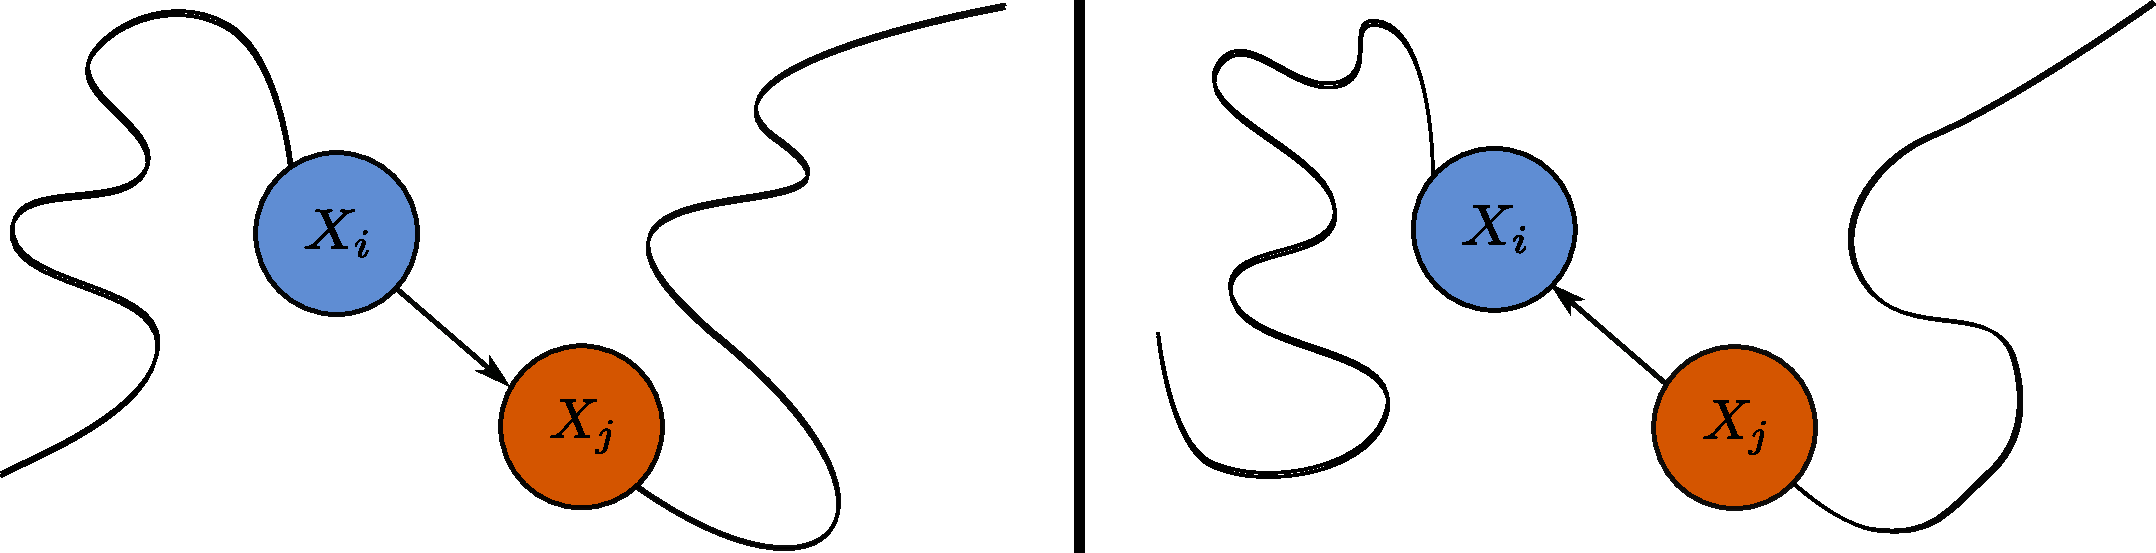
\includegraphics[width=0.75\textwidth]{imgs/mcmc1.pdf}
    \caption{Два состояния обратимой марковской цепи.}
    \label{fig:my_label}
\end{figure}
% \vspace*{1.5em plus .6em minus .5em}


\textbf{Доказательство}. Действительно, рассмотрим цепь с матрицей перехода $\mathbf{P}$ и начальным распределением $\lambda$:\\
$1) \Rightarrow 2)$. Пусть $n = 1$ :
\begin{equation}
    P(X_0 = i, X_1 = j) = P(X_0 = j, X_1 = i).
\end{equation}
Просуммируем по $j$:
\begin{equation}
    \sum_j P(X_0 = i, X_1 = j) = P(X_0 = i) = \lambda_i,
\end{equation}
\begin{equation}
    \sum_j P(X_0 = j, X_1 = i) = P(X_1 = i) = (\lambda \mathbf{P})_i.
\end{equation}
Таким образом, $\forall i$ $\lambda_i = (\lambda \mathbf{P})_i$ , т.е. $\lambda = (\lambda \mathbf{P} ) \Rightarrow $ цепь находится в состоянии равновесия со стационарным распределением $\lambda$. Далее,
\begin{equation}\begin{gathered}
    P(X_0 = i, X_1 = j) = P(X_1 = j | X_0 = i) P(X_0 = i) = p_{j i}\lambda_i = \\P(X_0 = j, X_1 = i) = P(X_1 = i | X_0 = j) P(X_0 = j) = p_{i j}\lambda_j,
\end{gathered}\end{equation}
т.е. имеет место условие сбалансированности.
$2) \Rightarrow 1)$. Перепишем
\begin{equation}
    P(X_0 = i_0, \dots, X_n = i_n) = \pi_{i_0}p_{i_0 i_1}\dots p_{i_{n-1} i_n}
\end{equation}
и воспользуемся уравнением (11):
\begin{equation}\begin{gathered}
    \pi_{i_0}p_{i_0 i_1}\dots p_{i_{n-1} i_n} = \pi_{i_1}p_{i_1 i_0}\dots p_{i_{n-1} i_n} = p_{i_1 i_0}\pi_{i_1}p_{i_1 i_2}\dots p_{i_{n-1} i_n} = \\p_{i_1 i_0}\pi_{i_2}p_{i_2 i_1}\dots p_{i_{n-1} i_n} = \dots = p_{i_1 i_0}p_{i_2 i_1}\dots \pi_{i_n}p_{i_n i_{n-1}} = \pi_{i_n} p_{i_n i_{n-1}}\dots p_{i_1 i_0} = \\P(X_0 = i_n, \dots, X_n = i_0) \blacktriangleright
\end{gathered}\end{equation}


Условие сбалансированности является сильным инструментом для нахождения стационарного распределения:

\begin{Th} Если $\lambda$ и $\mathbf{P}$ удовлетворяют уровнениям детального баланса
\begin{equation}
   \lambda_i p_{i j} = \lambda_j p_{j i},
\end{equation}
то $\lambda$ является стационарным распределением для $\mathbf{P}$, т.е. $\lambda \mathbf{P} = \lambda$.
\end{Th}

\textbf{Доказательство}. Просуммируем по $j$:
\begin{equation}
    \sum_j \lambda_i p_{i j} = \lambda_i \sum_j p_{i j} = \lambda_i,
\end{equation}
\begin{equation}
    \sum_j \lambda_j p_{j i} =  (\lambda \mathbf{P})_i.
\end{equation}
$\forall i$ выражения равны $\Rightarrow \lambda $ --- стационарное распределение и цепь обратима по теореме 2.$\blacktriangleright$
\[\] 

Таким образом, если для заданного распределения $p$ удастся найти такую матрицу перехода $\mathbf{P}$, что будет выполнено условие сбалансированности, то это распределение будет сходиться к стационарному с течением времени. 

\newpage
%{\LARGE \textbf{Метод Метрополиса-Гастингса \\в непрерывном случае}}\\
%\vspace*{1em plus .2em minus .2em}
   \subsection{Марковские цепи с непрерывным множеством состояний}	
Основные идеи Марковской цепи с дискретным пространством состояний могут быть обобщены на непрерывный случай.


\textit{Марковским процессом} $X_n$ c дискретным временем и множеством (уже не обязательно не более чем счетным) состояний $S$ будем называть такую последовательность, что

\begin{equation}
P(X_n \in A|X_{n-1} = x_{n-1},\dots,X_{0}=x_{0}) = P(X_n \in  A|X_{n-1} = x_{n-1}).
\end{equation}
Здесь $P(X_n \in A|X_{n-1}) = E(I_{X_n \in A}|X_{n-1} = x_{n-1})$ — условное математическое ожидание. 


Функция $P(X_n \in A|X_{n-1} = x_{n-1}) = p(x_{n-1}, A, n)$ называется переходной функцией марковского процесса, если $S \subset \mathbb{R}$. Если существует плотность $f_{X_n|X_{n-1}}(y|x)$, то она называется переходной плотностью $P_{x, y, n}$. 

\begin{figure}[H]
    \centering
    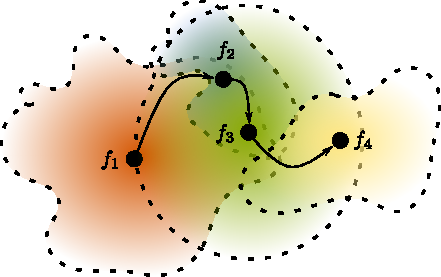
\includegraphics[width=0.65\textwidth]{imgs/blujd1.pdf}
    \caption{Визуализация марковского процесса: новое состояние зависит от плотности распределения ему предшествующего.}
    \label{fig:my_label}
\end{figure}
% \vspace*{1.5em plus .6em minus .5em} 


Рассмотрим стационарное распределение $\pi$ с переходной плотностью $P$, теперь уравнение Колмогорова - Чепмена \cite{fell} примет вид:
\begin{equation}
  \int_{x} \pi(x)P(x,y)dx= \pi(y).
\end{equation}


Обратимой назовем цепь, для которой выполняется уравнение детального баланса:
\begin{equation}
    P(x,y)p(x) = P(y,x)p(y).
\end{equation}


Опять условие сбалансированности влечет стационарность распределения. 


%\textbf{Теорема (эргодическая теорема для случая с непрерывным множеством состояний)}. Пусть $P(x,y)$ --- непрерывная положительная переходная плотность с множеством состояний $S$. Тогда $X_n$ сходится к единственному стационарному распределению.   
Из эргодической теоремы для случая с непрерывным множеством состояний \cite{Bellet} мы получаем, что распределение процесса сходится к стационарному.
\[\]

Тем самым, метод Монте-Карло будет работать и в случае марковских процессов с континуальным множеством состояний.
\[\]
Общая идея метода Монте-Карло Марковских цепей (MCMC):
\begin{itemize}
    \item построить цепь Маркова c эргодическим распределением, для которой стационарное распределение - это в точности заданное нами распределение,
    \item инициировать блуждание по цепи Маркова из некоторого начального состояния и дождаться, когда распределение сойдется к стационарному. С этого момента состояния цепи Маркова можно считать выборкой из желаемого распределения.
\end{itemize}






\newpage
%{\LARGE \textbf{Гиббсовское семплирование как частный случай Метрополиса-Гастингса}}\\
%\vspace*{1em plus .2em minus .2em}
\section{Гиббсовское семплирование}
\subsection{Идея и математическое обоснование}
В некоторых типах задач одномерные условные распределения гораздо легче моделировать, чем совместные распределения. Идея гиббсовского семплирования заключается в том, что для восстановления совместного распределения рассматриваются только условные распределения для каждой переменной. 
\\Для наглядности, рассмотрим двумерную случайную величину $(x,y)$. Мы хотим вычислить маргинальные распределения $p(x)$ и $p(y)$. Проще рассмотреть условные распределения $p(x|y)$, $p(y|x)$, чем искать совместную плотность посредством интегрирования $p(x) = \int p(x,y) dy$.
\\Семплирование начинается с некоторого значения $y_0$ для y. Генерируя случайную величину из условного распределения $p(x|y = y_0)$ получаем $x_0$. Далее используем $x_0$ для генерации нового значения $y_1$ из условного распределения $p(y|x = x_0)$. И так далее:
\begin{equation}
    x_i \sim  p(x|y = y_{i-1}), \ y_i \sim  p(y|x = x_i).
\end{equation}
Повторяя этот процесс k раз, получаем последовательность Гиббса длиной k с элементами $(x_j,y_j)$, $1 \leqslant j \leqslant k$. Последовательность Гиббса сходится к стационарному распределению, которое и является искомым.


Рассмотрим случай нескольких переменных: пусть явный вид распределения вычислить трудно, но известны условные плотности
\begin{equation}
    f_{X_i|X_1,\dots,X_{i-1},X_{i+1},\dots,X_n}({x_i|x_1,\dots,x_{i-1},x_{i+1},\dots,x_n}).
\end{equation}
Нам нужно сгенерировать вектор $(X_1,\dots,X_n)$, где мы знаем условные плотности.
\begin{itemize}
\item Выберем некоторый начальный вектор $(X_{1,1},\dots,X_{1,n})$, который вообще может \\получиться из нашего распределения.
\item Выберем случайный индекс $d$ из множества ${1,\dots,n}$.
%(почему марковость не ломается?)
\item Положим $X_{2,i} = X_{1,i}$ при $i \neq d$.
Величину $X_{2,d}$ сделаем случайной с плотностью $f_{X_d|X_1,\dots,X_{d-1},X_{d+1},\dots,X_n}({x_d|x_1,\dots,x_{d-1},x_{d+1},\dots,x_n})$.
\item Повторим шаг 2,3 для нового вектора и так далее.

\end{itemize}
Вектор $(X_{m,1},\dots,X_{m,n})$ сходится по распределению к требуемому вектору $(X_1,\dots,X_n)$ при $m\rightarrow\infty$.


Алгоритм на каждом шаге берет случайную величину и задает ее значение при фиксированных остальных.  
Таким образом, последовательно моделируются n случайных величин из n одномерных условных выражений вместо того, чтобы генерировать один n-мерный вектор за один подход с использованием полного совместного распределения. Последовательность генерируемых значений образует обратимую цепь маркова, эргодическое распределение которой является искомым.
\[\]

Убедимся, что алгоритм гиббсовского семплирования укладывается в изложенную \\теорию.\\
В данном случае мы рассматриваем процесс с переходной плотностью из $\vec{x} = (x_1,\dots,x_n)$ в $\vec{y} = (x_1,\dots,x_{k-1},z,x_{k+1},\dots,x_n)$.
\begin{equation}
    P(\vec{x}, \vec{y})=\frac{1}{n} f_{X_{k} | X_{1}, \ldots, X_{k-1}, X_{k+1}, \ldots, X_{n}}\left(z | x_{1}, \ldots, x_{k-1}, x_{k+1}, \ldots, x_{n}\right).
\end{equation}

Проверим, что она удовлетворяет условию сбалансированности с нужной нам $p(\vec{x}) = f_{X_1,\dots, X_n}(\vec{x})$.
Действительно,
\begin{equation}
    P(\vec{x}, \vec{y}) p(\vec{x})=\frac{1}{n} \frac{f_{X_{1} \ldots, X_{n}}\left(x_{1} \ldots, x_{k-1}, z, x_{k+1}, \ldots, x_{n}\right)}{f_{X_{1} \ldots X_{k-1}, X_{k+1}, \ldots, X_{n}}\left(x_{1}, \ldots, x_{k-1}, x_{k+1}, \ldots, x_{n}\right)} f_{X_{1}, \dots, X_{n}}\left(x_{1},., x_{n}\right).
\end{equation}
При этом $P(\vec{y}, \vec{x}) p(\vec{y})$ даст ту же формулу с точностью до перестановки множителей.
Следовательно, построенная цепь является сбалансированной с нужной плотностью.

\newpage
%{\LARGE \textbf{Гиббсовское семплирование}}\\
%\vspace*{1em plus .2em minus .2em}
%\section{Задача}
\subsection{Задача про одинаково распределенные точки в круге}

Предположим, что мы хотим взять наугад выборку из $N$ точек в единичном круге, удаленных друг от друга не менее чем на расстояние $d$. Выписать для данной задачи совместную плотность вектора трудно, однако условные плотности устроены довольно просто. Eсли мы знаем все точки, кроме одной, то оставшаяся точка распределена равномерно на исходном круге за вычетом кругов радиуса $d$ вокруг остальных точек.
\[\]
Следуя алгоритму гиббсовского семплирования :
\begin{itemize}
    \item На первом шаге мы случайным образом выбираем точку в исходном круге радиуса 1 $U_1$. Назовем эту точку $X_1$. Пусть $U_d(X_1)$---круг радиуса $d$ с центром в точке $X_1$. Вторая точка выбирается случайно из множества $U_1 \setminus U_d(X_1)$. Третья точка $X_3$ выбирается случайно из множества $U_1 \setminus U_d(X_1)\setminus U_d(X_2)$. И так далее.
    \item Дальше мы генерируем случайный индекс $i$ и меняем элемент $X_i$ нашей выборки $(X_1, \dots, X_N)$ на точку, равномерно распределённую в единичном круге без остальных $N-1$ кругов радиусов $d$. После большого числа итераций полученный набор из $N$ точек будет иметь искомое распределение.
\end{itemize}

\begin{figure}[H]
    \centering
    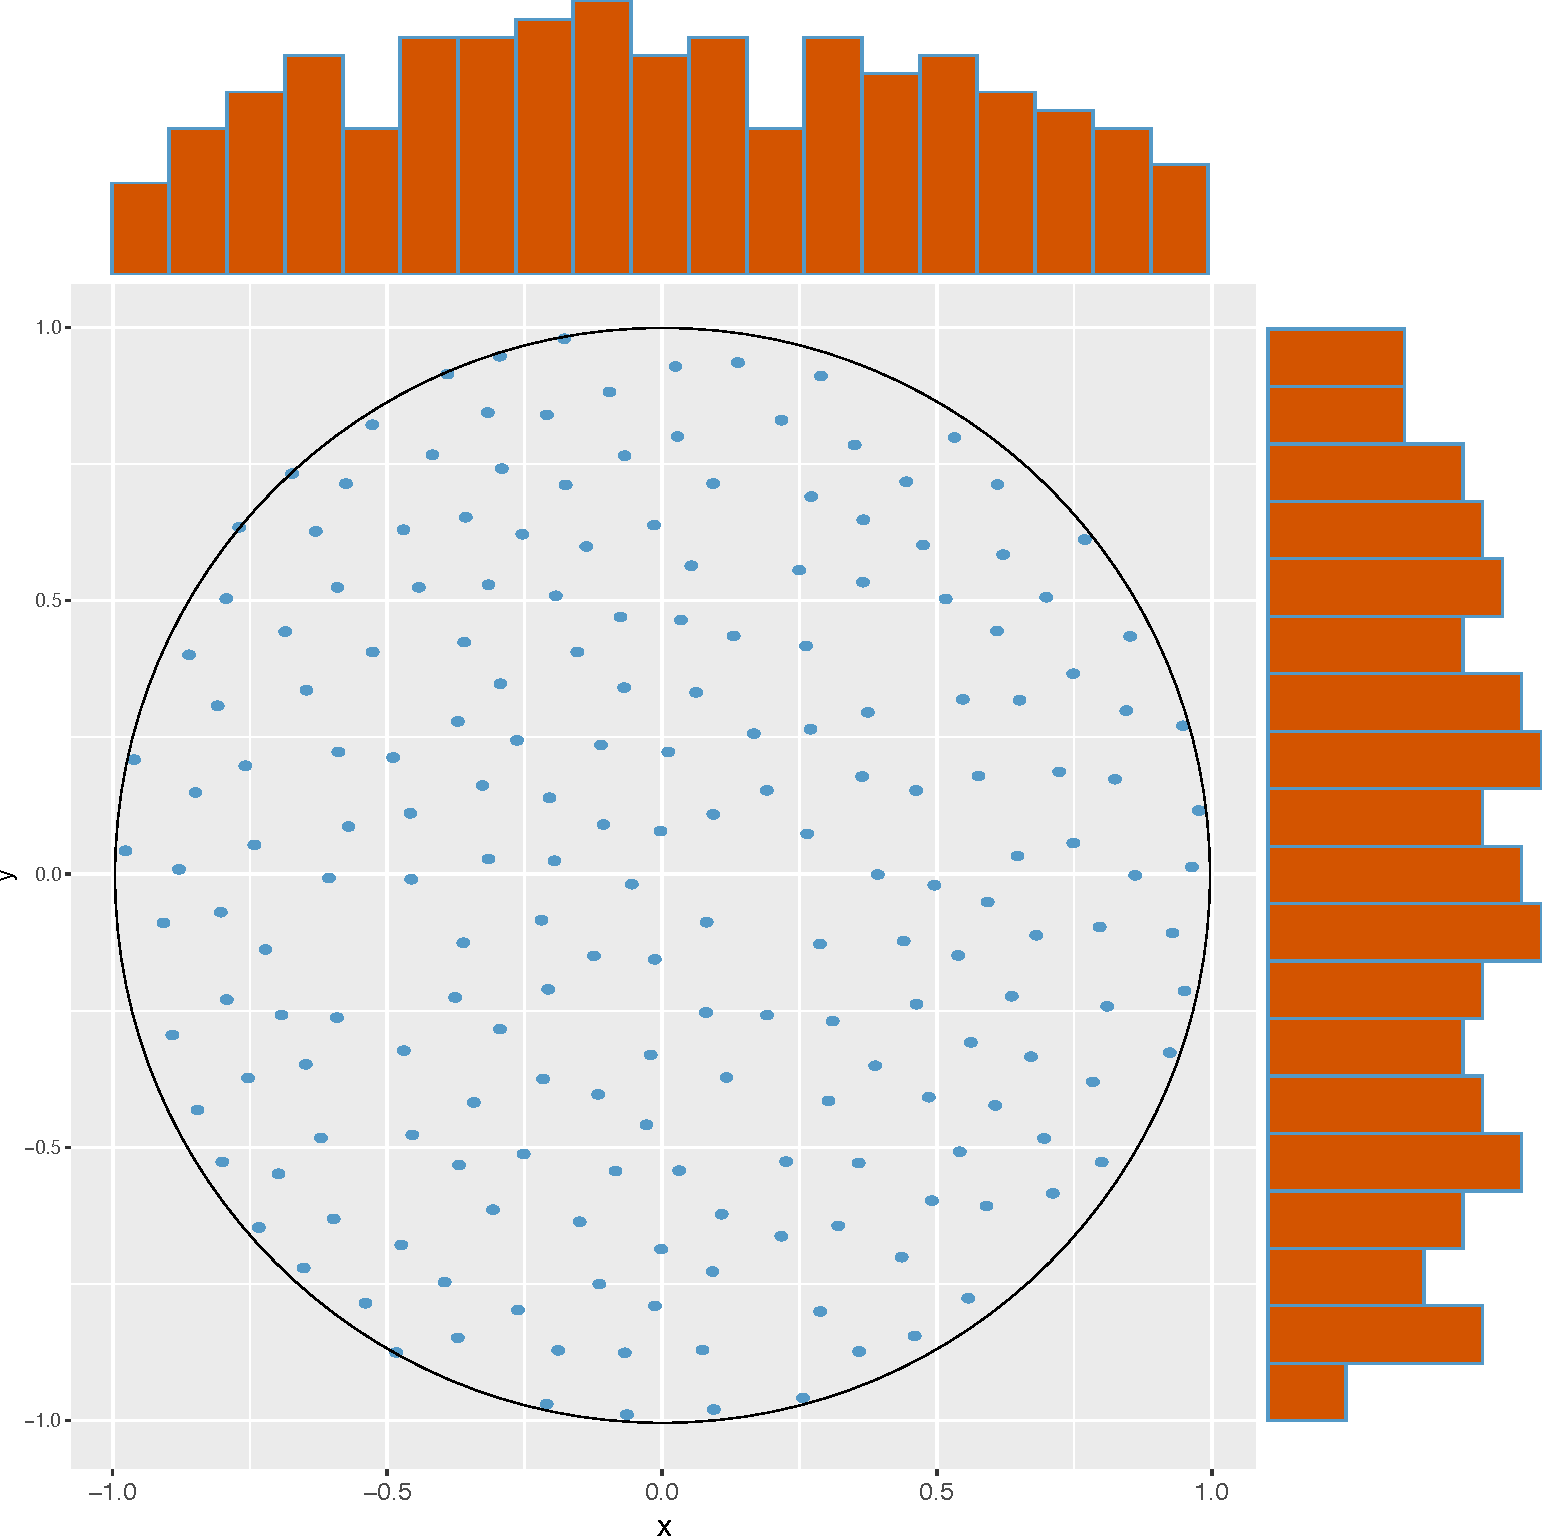
\includegraphics[width=0.65\textwidth]{imgs/RplotGRU.pdf}
    \caption{Равномерное распределение точек в круге.}
    \label{fig:my_label}
\end{figure}

Если мы не будем использовать гиббсовское семплирование, то уже вторая сгенерированная точка не будет попадать в центр круга, поскольку её будет вытеснять равномерно - распределённая первая точка. Значит, первая и вторая точки не будут одинаково распределены.


Чтобы это заметить, пронаблюдаем распределение первой и второй брошенных в круг точек при гиббсовском семплировании и без (рис.7. и рис. 8.).
\begin{figure}[H]
   \begin{minipage}{0.52\textwidth}
     \centering
     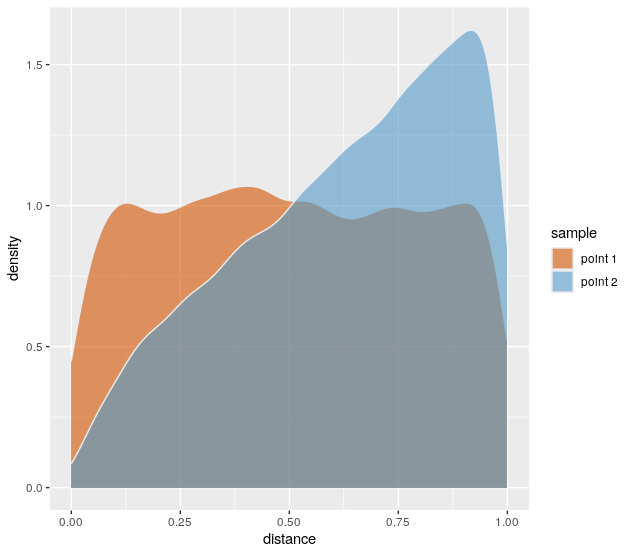
\includegraphics[width=1\linewidth]{imgs/Rplot01.png}
     \caption{Распределения точек без семпирования.}\label{Fig:Data1}
   \end{minipage}\hfill
   \begin{minipage}{0.52\textwidth}
     \centering
     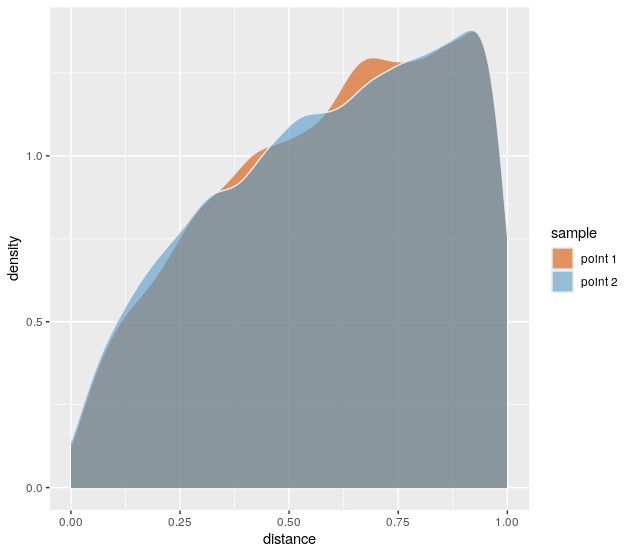
\includegraphics[width=1\linewidth]{imgs/Rplot05.png}
     \caption{Распределения с семплированием.}\label{Fig:Data2}
   \end{minipage}
\end{figure}

Для данной работы алгоритм гиббсовского семплирования и графики были реализованы с помощью языка программирования $R$. Код доступен по ссылке \cite{code}. Иллюстрации выполнены в графическом редакторе Inkscape.
\newpage
%\section{Вывод.}
\addcontentsline{toc}{section}{Вывод}
\section*{Вывод}
Мы показали, что можно построить марковскую цепь с заранее заданным эргодическим распределением. В эту теорию укладывается метод гиббсовского семплирования, который позволяет моделировать совместное распределение, используя только условные, что облегчает вычисления во многих задачах. Например, в рассмотренной задаче заполнения круга одинаково распределенными точками использование гиббсовского семплирования позволяет восстановить искомое распределение, исходя из условных плотностей. Задача восстановления данных имеет ту же структуру: совместное распределение посчитать сложно, но условные распределения приблизительно известны. Таким образом, изученный алгоритм может быть использован для решения задачи восстановления данных.



\newpage
\addcontentsline{toc}{section}{Приложения}
\section*{Приложения}
\begin{minted}{R}
library(hexbin)
library(RColorBrewer)
library(ggplot2)
library(ggExtra)

rcircle = function(r=1){
  r = r * sqrt(runif(1))
  theta = runif(1) * 2 * pi
  
  x = r * cos(theta)
  y = r * sin(theta)
  return(c(x,y))
}

start <- function(N_points, r, d){
  start_samp <- matrix(-r*100, N_points, 2) #Generate points far away from center
  
  A = rcircle(r)
  x1 <- A[1]
  y1 <- A[2]
  i = 1
  j = 1
  k = 0 #flag for searching the right second point
  c=0
  
  for (i in 1:N_points){
    #the second point's generation
    while (k == 0){
      A = rcircle(r)
      x2 <- A[1]
      y2 <- A[2]
    
      c = c+1
      #If we cant generate point for 10 000 times - break
      if (c == 10000){ 
        warning("Generation timed out")
        return()
      }
      
      #the distance between current point and all that we've already taken
      for (j in 1:N_points){
        x_sq = (start_samp[j,1] - x2)^2
        y_sq = (start_samp[j,2] - y2)^2
        distance = sqrt(x_sq + y_sq)
        
        if (distance < d){
          k = 0
          break
        }
        #if we didn't get into the previous 'if' conditions => our 2nd point is correct and then flag k = 1, 
        #if we got into this conditions then 'break' operator will stop it and there will be selected new x2, y2.
        k = 1
      }
    }
    start_samp[c(i), 1] <- x2
    start_samp[c(i), 2] <- y2
    k = 0
  }
  return(start_samp)
}

sampling <- function(start_samp, r, d, N_samling = 100, silent = T){
  j = 1
  k = 0
  m = 1
  c=0
  
  N_points = NROW(start_samp)
  if (!silent)
    pb = txtProgressBar(min = 0, max = N_samling, style = 3) #fashion progressbar
  for (m in 1:N_samling){
    if (!silent)
      setTxtProgressBar(pb,m)
    
     current = sample(1:N_points, 1) #random index

    #the second point's ganeration
    while (k == 0){
      
      A = rcircle(r)
      xi <- A[1]
      yi <- A[2]
     
      #the distance between current point and all that we've already taken
      for (j in 1:N_points){
        if ( j != current){
         
          x_sq = (start_samp[j,1] - xi)^2
          y_sq = (start_samp[j,2] - yi)^2
          distance = sqrt(x_sq + y_sq)
          
          if ( distance < d){
            k = 0
            break
          }
          k = 1
        }
      }
    }
    start_samp[current, 1] = xi
    start_samp[current, 2] = yi
    k = 0
  }
  if (!silent)
    close(pb)
  
  return(start_samp)
}

D = 0.9
R = 1
N_POINTS = 2
N_SAMPLING = 1e4

  A = start(N_points = N_POINTS, r = R, d = D)
  plot(A[,1], A[,2], pch=16, ylim=c(-1,1), xlim=c(-1,1))

  A_resampled= sampling(A, r = R, d = D, N_samling = N_SAMPLING)
  
#------------------------ 
  plot(A_resampled[,1], A_resampled[,2], pch=16)
  library(ggplot2)
  library(ggExtra)
  
  d1 <- as.data.frame(A_resampled, stringsAsFactors=FALSE)
  x <- d1[,1]
  y <- d1[,2]
  
  p <- ggplot(d1, aes(x=x, y=y)) +
    geom_point(fill="slateblue",col="#5499c7") +
    theme(legend.position="none")
  p
  # with marginal histogram
  p1 <- ggMarginal(p, type="histogram", fill = "#d35400",col = "#5499c7", size = 3, xparams = list(  bins=20), yparams = list(  bins=20))
  p1
#------------------
  STOP = 1e4
  D = 1
  R = 1
  N = 2
  Nsamp = 100
  
  nosamp_matr =start(N_points = N_POINTS, r = R, d = D)
  samp_matr = sampling(A,r = R, d = D, N_samling = Nsamp)
  
  PB = txtProgressBar(min = 0, max = STOP, style = 3)
  
  for (i in 1:(STOP - 1)){
    setTxtProgressBar(PB, i)
    
    A = start(N_points = N, r = R, d = D)
    nosamp_matr = cbind(nosamp_matr, A)
    B = sampling(A,r = R, d = D, N_samling = Nsamp)
    samp_matr = cbind(samp_matr, B)
  }
  
  fir = matrix(samp_matr[1,], byrow = T, ncol = 2)
  sec = matrix(samp_matr[2,], byrow = T, ncol = 2)
  
  fir_NO = matrix(nosamp_matr[1,], byrow = T, ncol = 2)
  sec_NO = matrix(nosamp_matr[2,], byrow = T, ncol = 2)
  
  dist1 = data.frame(abs(fir[,1]^2+fir[,2]^2))
  dist2 = data.frame(abs(sec[,1]^2+sec[,2]^2))
  names(dist1) = "dist"
  names(dist2) = "dist"
  dist1$name = "dist1"
  dist2$name = "dist2"
      
  df = rbind(dist1, dist2)
  names(df) = c("dist", "sample")
  ggplot(df, aes(dist, fill = sample)) + geom_histogram(color="#e9ecef",alpha = 0.6, position = "identity")+scale_fill_manual(values=c("#d35400", "#5499c7"))
  ggplot(df, aes(dist, fill = sample)) + geom_density(color="#e9ecef",alpha = 0.6)+scale_fill_manual(values=c("#d35400", "#5499c7"))

  dist1_NO = data.frame(abs(fir_NO[,1]^2+fir_NO[,2]^2))
  dist2_NO = data.frame(abs(sec_NO[,1]^2+sec_NO[,2]^2))
  names(dist1_NO) = "dist"
  names(dist2_NO) = "dist"
  dist1_NO$name = "dist1"
  dist2_NO$name = "dist2"
  
  df = rbind(dist1_NO, dist2_NO)
  names(df) = c("dist", "sample")
  ggplot(df, aes(dist, fill = sample)) + geom_histogram(color="#e9ecef",alpha = 0.6, position = "identity")+scale_fill_manual(values=c("#d35400", "#5499c7"))
  ggplot(df, aes(dist, fill = sample)) + geom_density(color="#e9ecef",alpha = 0.6)+scale_fill_manual(values=c("#d35400", "#5499c7"))
\end{minted}

\newpage

\begin{thebibliography}{3}
\bibitem{la}
Муромцева, Г. А., et al. Распространенность факторов риска неинфекционных заболеваний в российской популяции в 2012-2013гг. Результаты исследования ЭССЕ-РФ. Кардиоваскулярная терапия и профилактика 13(6) (2014).

\bibitem{b}
Buuren, S. V., & Groothuis-Oudshoorn, K. Mice: Multivariate imputation by chained equations in R. Journal of statistical software (2010).

\bibitem{phys}
Metropolis, N., & Ulam, S. The monte carlo method. Journal of the American statistical association, 44(247) (1949). 

\bibitem{fell}
Феллер, В. Введение в теорию вероятностей и ее приложения (Vol. 2). Рипол Классик (2013).

\bibitem{kelb}
Кельберт, М., & Сухов, Ю. Вероятность и статистика в примерах и задачах. Том 2. Марковские цепи как отправная точка теории случайных процессов и их приложения. Litres (2017).

\bibitem{Murphy}
Murphy, K. P. Machine learning: a probabilistic perspective. MIT press (2012).

\bibitem{shir}
Ширяев, А. Н. Вероятность. В 2-х кн. Москва: МЦНМО (2004).

\bibitem{Bellet}
Bellet, L. R. Ergodic properties of Markov processes. In Open quantum systems II (pp. 1-39). Springer, Berlin, Heidelberg (2006). 

\bibitem{code}
\url{https://github.com/annalimm/Gibbs_circle.git}.
\end{thebibliography}
  

\end{document}  


